\newcommand{\archerDescription}{
\section{Archer}
    Dedicated to his ranged craft, an archer is often precise and meticules.
    Although he can be a hunter, he can also very well be a noble, shooting only
    in tournaments, rarely setting a foot outside the city walls.
    It goes witout saying that an archer trains with ranged weapons, thus Ranged
    is a career skill. If you can't see your target you surely can't hit it, thus
    an archer is often perceptive. Discipline is needed to for that inner focus
    to hit that tiny spot in the distance. Finally in the heat of the moment, he
    needs to keep his Cool, so that he does not let his projectile fly too early.\\
    \\
    See \nref{tlttree:archer} for more information.
}

\newcommand{\archerTree}{
    \newpage
    \subsection{Archer Talent Tree}
    \label{tlttree:archer}

    \textbf{Class Skills:} Athletics, Cool, Crafting, Perception, Ranged, Discipline
    \newline

    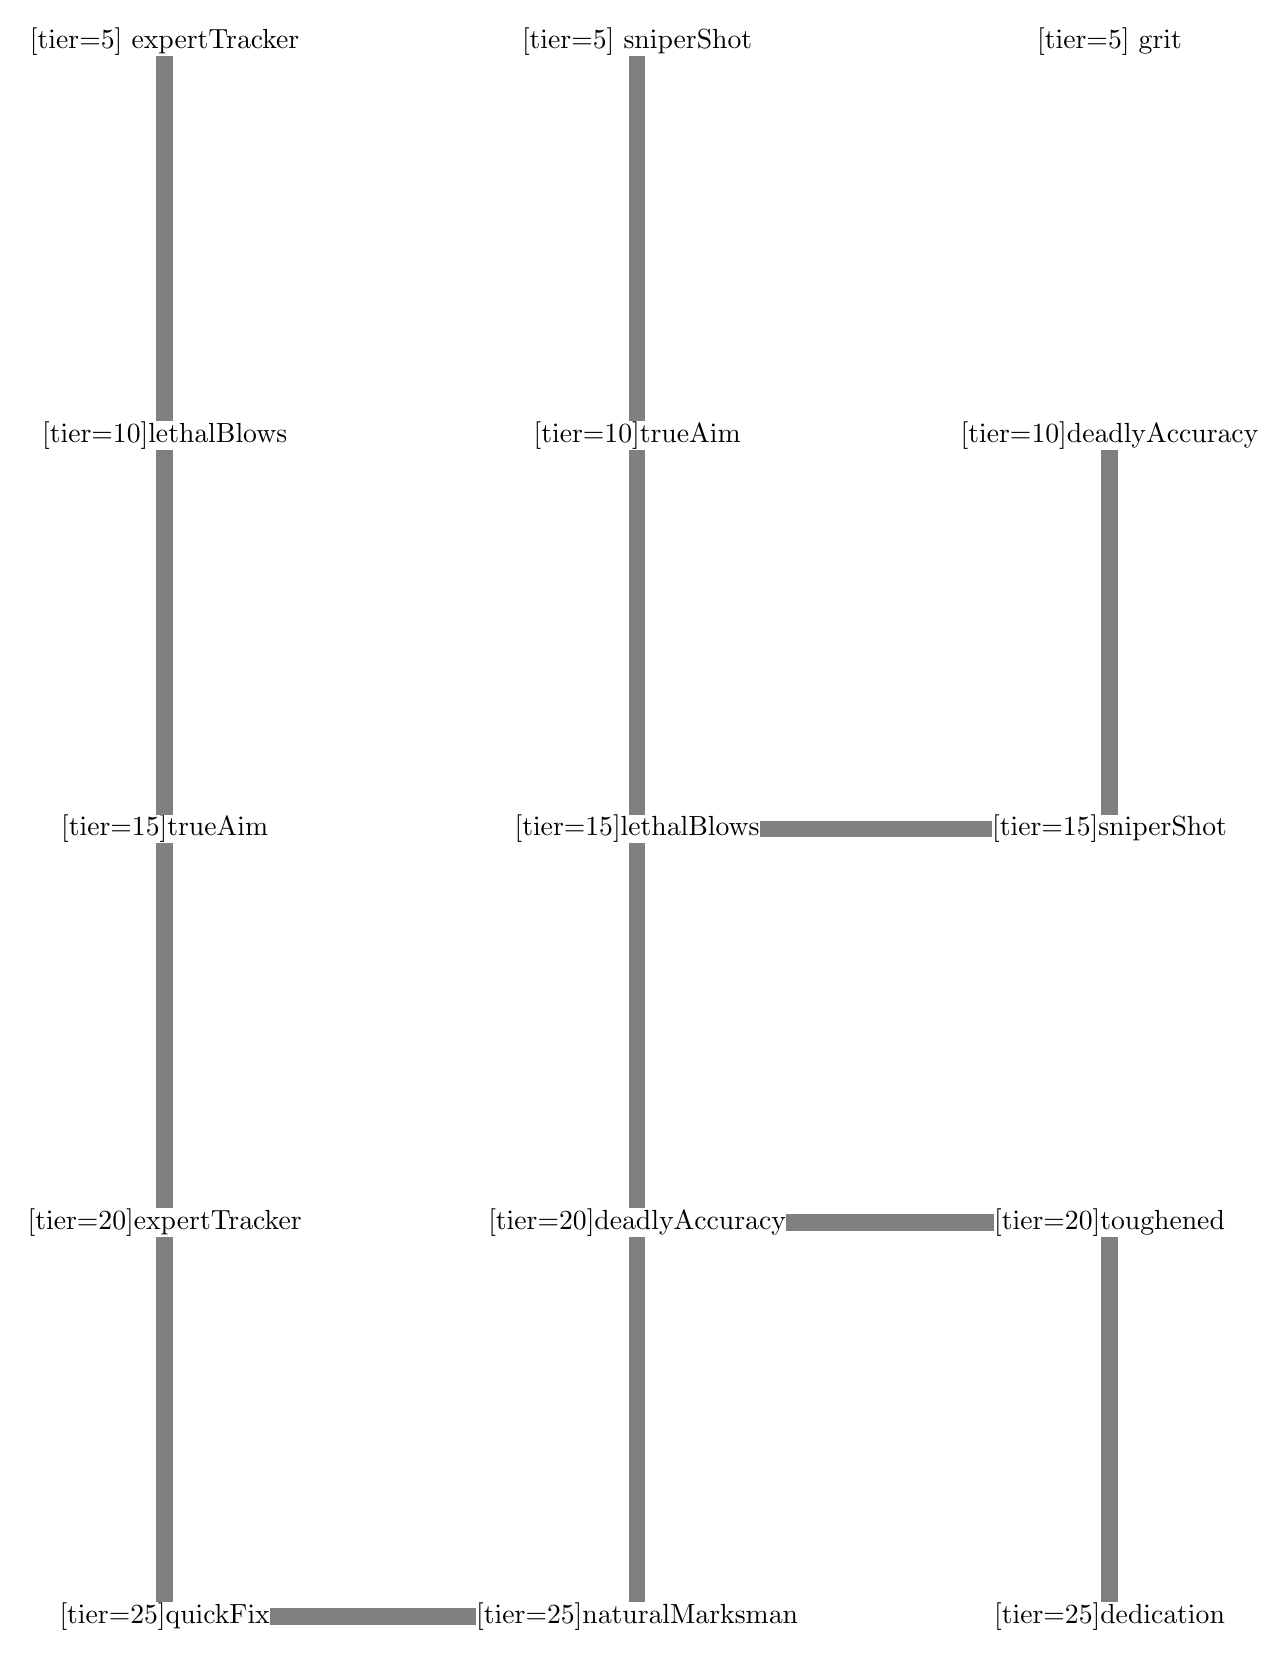
\begin{tikzpicture}
        \draw ( 0,  0) node(aa)[inner sep=0]{\TalentBox[tier=5] {expertTracker}}
              ( 6,  0) node(ab)[inner sep=0]{\TalentBox[tier=5] {sniperShot}}
              (12,  0) node(ac)[inner sep=0]{\TalentBox[tier=5] {grit}}
              ( 0, -5) node(ba)[inner sep=0]{\TalentBox[tier=10]{lethalBlows}}
              ( 6, -5) node(bb)[inner sep=0]{\TalentBox[tier=10]{trueAim}}
              (12, -5) node(bc)[inner sep=0]{\TalentBox[tier=10]{deadlyAccuracy}}
              ( 0,-10) node(ca)[inner sep=0]{\TalentBox[tier=15]{trueAim}}
              ( 6,-10) node(cb)[inner sep=0]{\TalentBox[tier=15]{lethalBlows}}
              (12,-10) node(cc)[inner sep=0]{\TalentBox[tier=15]{sniperShot}}
              ( 0,-15) node(da)[inner sep=0]{\TalentBox[tier=20]{expertTracker}}
              ( 6,-15) node(db)[inner sep=0]{\TalentBox[tier=20]{deadlyAccuracy}}
              (12,-15) node(dc)[inner sep=0]{\TalentBox[tier=20]{toughened}}
              ( 0,-20) node(ea)[inner sep=0]{\TalentBox[tier=25]{quickFix}}
              ( 6,-20) node(eb)[inner sep=0]{\TalentBox[tier=25]{naturalMarksman}}
              (12,-20) node(ec)[inner sep=0]{\TalentBox[tier=25]{dedication}}
        ;

        \tikzstyle{bar}=[gray,-,>=stealth, line width=6pt]

        \draw [bar] (aa) to (ba);
        \draw [bar] (ab) to (bb);

        \draw [bar] (ba) to (ca);
        \draw [bar] (bb) to (cb);
        \draw [bar] (bc) to (cc);

        \draw [bar] (ca) to (da);
        \draw [bar] (cb) to (db);

        \draw [bar] (da) to (ea);
        \draw [bar] (db) to (eb);
        \draw [bar] (dc) to (ec);

        \draw [bar] (cb) to (cc);

        \draw [bar] (db) to (dc);

        \draw [bar] (ea) to (eb);
    \end{tikzpicture}
}
